\chapter{Unity Application}
The Unity application is the visualization of the digital twin and the world around it.

\section{Modes}
The application can be run in three modes. The first mode, Sim Mode, retrieves data from the ReVolt Simulator to visualize. This mode is useful for visualizing ReVolt, when the ReVolt model is not available. This mode was also useful in development of the application without needing continual access to ReVolt.

The second mode, Twin Mode, retrieves data directly from the ReVolt model through the Azure IoT Hub. In this mode, the application and the ReVolt model are functioning together. Information about the position and orientation of the boat, the position of real world obstacles and other relevant information is sent to the application. At the same time, information about virtually placed objects/obstacles and control commands are sent to the ReVolt model. This mode can be used to test the model with virtual objects, to visualize ReVolt and it's environment from a remote location, and to save information in the IoT Hub for later reference.

The third mode, Playback Mode, retrieves stored data from the IoT Hub to playback previous scenarios. This can be useful in replaying and analyzing a fault scenario, a specific test case or using specific environment conditions. The stored data is retrieved from the Azure IoT SQL Databases.

\section{Virtual ReVolt}

The virtual ReVolt in the Unity Application is the visualization of the digital twin. It is comprised of 2 computer models. The first model is a detailed CAD model of ReVolt imported into Unity ( \Cref{fig:detailedReVoltModel}). This model keeps the aesthetics and details of the boat. The second is a simplified model that is overlaid onto the detailed model, but is not visible ( \Cref{fig:SimplifiedReVoltModel}). This model serves a dual purpose. First, if any large physics calculations need to be done in the Unity Application, this would not be reasonable on the detailed model, but can be easily done on the simplified model. The second purpose of the simplified model is to function as an indicator to collisions, as it will turn red during collisions.

\begin{figure}[H]
\centering
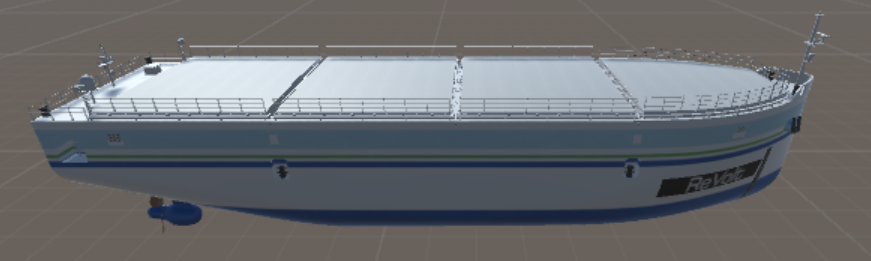
\includegraphics[scale=0.5]{Images/DetailedModel.png}
\caption{Detailed ReVolt model exported to Unity}
\label{fig:detailedReVoltModel}
\end{figure}

\begin{figure}[H]
\centering
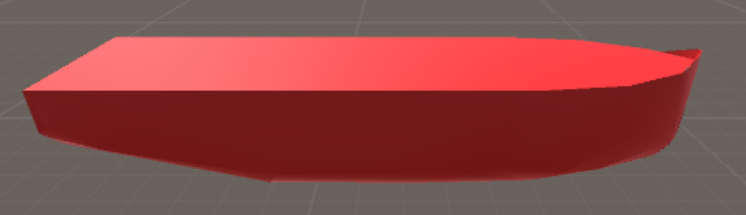
\includegraphics[scale=0.6]{Images/SimplifiedModel.png}
\caption{Simplified ReVolt model exported to Unity}
\label{fig:SimplifiedReVoltModel}
\end{figure}

\section{Virtual World}
The virtual world around ReVolt in the Unity Application consists of several types of objects. The ocean is the main feature of the world. It is surrounded by land features, including rocky coasts and docks. Obstacle boats can also be included in the virtual world. Each object has certain data associated with it to correctly place the object in the world (position, orientation, size, etc.).

A virtual world object (e.g. boat, dock, land, etc.) can be generated from one of three sources. First, the data regarding the object can come from the ReVolt model, who has sensed the object and streams the information back to the application through the Azure IoT Hub. Second, the data regarding the object can be send from the ReVolt Simulator. These objects are handled in the same way as objects generated from the ReVolt model.

Third, the virtual world can include objects a user can generate in the Unity application. The data regarding the these objects are streamed to the ReVolt model. These objects, generated in the application, are meant to be treated as actual obstacles by the ReVolt model. This feature can be taken advantage of in order to test obstacle avoidance algorithms without a sensing system for the obstacle in the loop and also without the risk of an actual collision. 

%The virtual world around ReVolt in the Unity Application consists of both real objects that are conveyed from ReVolt (either the model or the simulation) and virtual objects which do not exist in real life, but are transmitted to ReVolt to inform its decision making. This can be useful for testing specific maneuvers around other boats, without having to risk a crash.

In Sim Mode, the ocean data available is quite exact, so the ocean in the Unity Application is adjusted to follow the movements of the simulated ocean. The ocean parameters can be tuned in the ReVolt simulator for testing in various ocean conditions. However, when using data collected from the model ReVolt, it is not possible to accurately represent the motion of the waves.

\todo[inline]{Obstacle image}
\todo[inline]{Ocean image}
\todo[inline]{Land image}